% 招聘状ジェネレータ
% by Akinori Ito, 2018/8/12
%
\documentclass[12pt]{article}
\usepackage{graphicx}
\usepackage{mediabb}
\usepackage{color}
\evensidemargin=-1in
\oddsidemargin=-1in
\topmargin=-1.8in
\textwidth=210mm
\textheight=297mm
\pagestyle{empty}
\long\def\fixedbox#1#2#3{\vbox to #2{\parbox[t]{#1}{#3}\vfil}}
\long\def\fixedhbox#1#2#3{\parbox[t]{#1}{\vbox to #2{#3\vfil}}}
\def\schedline#1#2#3#4{\small%
\fixedhbox{4.1cm}{1cm}{#1}\hspace{0.1cm}
\fixedhbox{4.1cm}{1cm}{#2}\hspace{0.1cm}
\fixedhbox{4.1cm}{1cm}{#3}\hspace{0.1cm}
\fixedhbox{4.1cm}{1cm}{#4} \\[0.8mm]}
\newlength\letterheadheight

%%%個別の書類についての記述事項ここから
%%%招聘する相手の情報

% ※招聘者と身元保証人が同じ場合にしか対応していません
%  個別に指定する場合は各自なんとかしてください

% 書類作成日
\def\平成{30}
\def\西暦{2018}
\def\月{8}
\def\月英語{August}
\def\日{13}

% 書類提出先 必要ない場合は空欄
% 記載する場合は大使か総領事のどちらかにチェックマークを入れてもう片方は空欄にする
\def\大使館存在国{中華人民共和国} %あるいは「上海」とか
\def\大使{V}
\def\総領事{V}

% 招聘される人の情報
\def\国籍{相手の国籍}
\def\職業{XXX大学教授}
\def\氏名{相手の名前}
\def\所属{XXX University}
\def\称号{Prof.}
% 男か女のどちらかにチェックを入れてもう片方は空欄にする
\def\男{V}
\def\女{V}
\def\生年{1900}
\def\生月{12}
\def\生日{31}
\def\年齢{55}

% 著者と題目は後の目的と経緯に利用しているので、必要なければ省略可
\def\著者{著者リスト}
\def\題目{Title of the paper}

% スケジュール
% 年月日、予定、連絡先、滞在先を記載
\def\スケジュール{
\schedline{2018年12月22日}{北京から仙台に飛行機で移動}{実行委員長 090-1234-5678}{仙台のホテル} 
\schedline{2018年12月23日}{仙台で国際会議ICXXX2018に参加}{同上}{仙台のホテル}
\schedline{2018年12月24日}{同上}{同上}{仙台のホテル}
\schedline{2018年12月25日}{同上}{同上}{仙台のホテル}
\schedline{2018年12月26日}{仙台から北京に飛行機で移動}{同上}{}
}

%%% イベントごとに変える情報

% 招聘目的、経緯、関係
\def\目的{\small
ビザ申請人は、2018年12月23日から25日まで宮城県仙台市で開催される国際会議International Conference on X-ray eXamination on Xmas (ICXXX 2018)で研究成果を発表する。}
\def\経緯{\small
ビザ申請人は、論文``\題目'' (著者\著者)を上記国際会議に投稿し、審査の結果採択され、当該国際会議にて発表することになった。}
\def\関係{当該国際会議実行委員長と参加者の関係である。}

% 招聘者の情報
\def\招聘者氏名{伊藤 彰則}
\def\招聘者郵便番号1{980}
\def\招聘者郵便番号2{0000}
\def\招聘者住所{仙台市青葉区中央1丁目1-1}
\def\招聘者所属{青葉山工業大学 教授}
\def\招聘者電話{022-1234-5678}
\def\招聘者FAX{080-1234-5678}
\def\招聘者誕生年{1964}
\def\招聘者誕生月{1}
\def\招聘者誕生日{1}
\def\招聘者年齢{54}


% 招待状のレターヘッドのファイル(PDF)
\def\letterheadfile{letterhead.pdf}
% レターヘッドの高さ
\letterheadheight=5cm

%招待状の文面
\long\def\招待状{
\quad Thank you for registering for The N-th International Conference on X-ray eXamination on Xmas 
 (ICXXX 2018), which will be held in Sendai, Miyagi, Japan, during 23-25 December, 2018. 

\quad We are proud to invite you as a speaker/participant in the symposium and are looking 
forward to your presentation/discussion. Details of the program are published on the 
ICXXX 2018 website at http://icxxx2018.fake/. The site also contains information for travel to the conference venue. 
The conference will be held 
in Sendai, Japan. Please make arrangements for your travel. Once again, congratulations for 
your excellent work. We look forward to seeing you at ICXXX 2018.
\bigskip
 
Sincerely yours,   
          
\bigskip        
\hspace{6cm}\parbox{10cm}{                                                                                         
\begin{flushleft}   
Akinori Ito, Professor \\ 
General Chair of ICXXX 2018 \\ 
Graduate School of Engineering \\ 
Aobayama Institute of Technology \\
6-6-5 Aramaki aza Aoba, Aoba-ku, Sendai, Miyagi \\
980-8579, JAPAN. 
\end{flushleft}
}
}

%%%個別の書類についての記述事項ここまで

\begin{document}
%\color{red}
\vbox to 0in {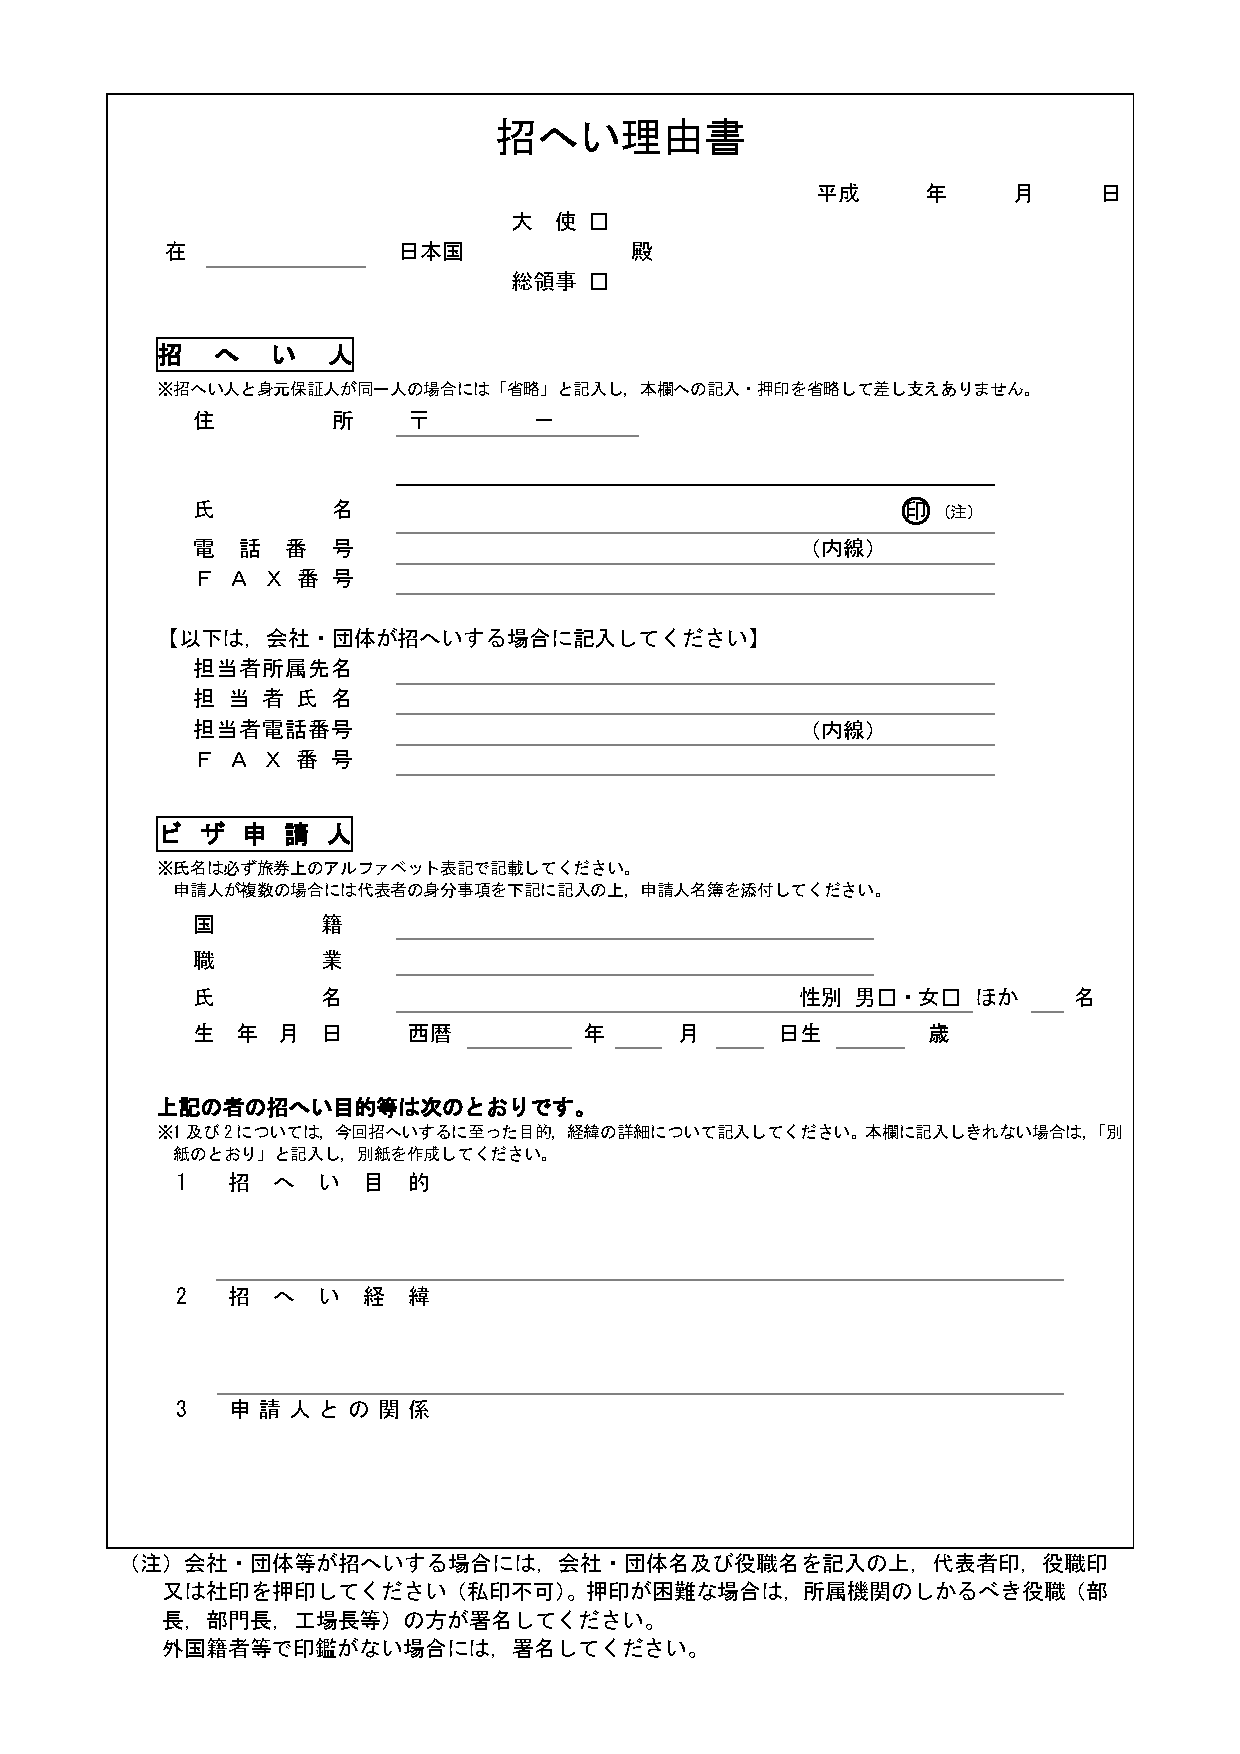
\includegraphics{000262560.pdf}}
\vspace{2.9cm}
\hspace{15cm}\平成\hspace{1.3cm}\月\hspace{1.1cm}\日 \hfill \\
\hspace{10.6cm}\大使 \hfill\\
\hspace{4.3cm}\hbox to 2cm{\大使館存在国\hfil} \hfill \\
\hspace{10.6cm}\総領事 \hfill\\
\ \\[2.9cm]
\hspace{8cm}省略\\
\ \\[5.9cm]
\hspace{7.5cm}\国籍\\[0.13cm]
\hspace{7.5cm}\職業\\[0.13cm]
\hspace{7,5cm}\hbox to 6cm{\氏名\hfil}\hspace{2cm}\hbox to 1.1cm{\男\hfil}\hbox to 1.1cm{\女\hfil}\\[0.13cm]
\hspace{9cm}\生年\hspace{0.9cm}\hbox to 1cm{\hfil\生月}\hspace{0.6cm}\hbox to 1cm{\hfil\生日}\hspace{1.7cm}\年齢\\
\ \\[2cm]
\hspace{4cm}\fixedbox{14cm}{1.5cm}{\目的}\\[0.4cm]
\hspace{4cm}\fixedbox{14cm}{1.5cm}{\経緯}\\[0.4cm]
\hspace{4cm}\fixedbox{14cm}{1.5cm}{\関係}\\

\clearpage

\vbox to 0in{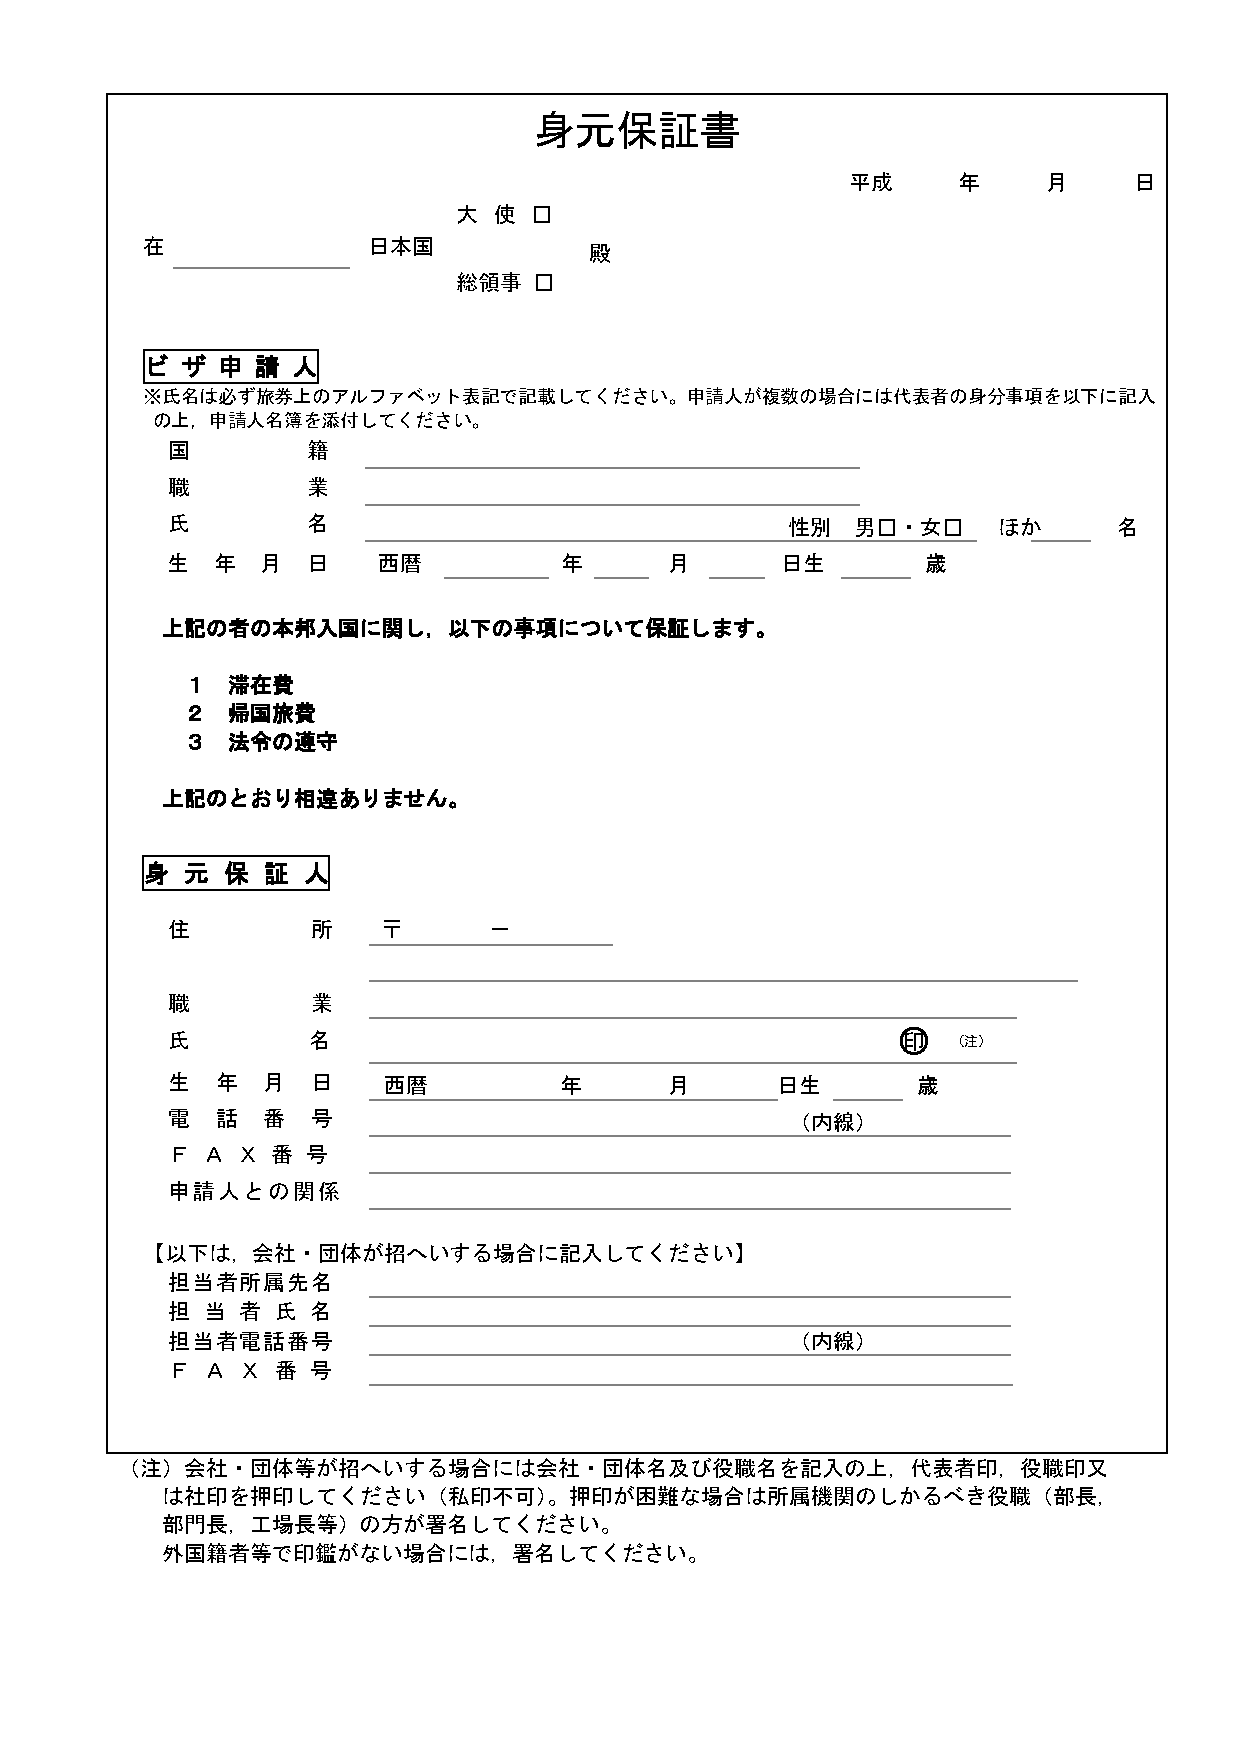
\includegraphics{000262559.pdf}}
\vspace{2.7cm}
\hspace{15.5cm}\平成\hspace{1.3cm}\月\hspace{1.1cm}\日 \hfill \\[0.07cm]
\hspace{9.7cm}\大使 \hfill\\[0.07cm]
\hspace{4.1cm}\hbox to 2cm{\大使館存在国\hfil} \hfill \\[0.07cm]
\hspace{9.7cm}\総領事 \hfill\\[0.07cm]
\ \\[1.8cm]
\hspace{7cm}\国籍\\[0.13cm]
\hspace{7cm}\職業\\[0.13cm]
\hspace{7cm}\hbox to 6.2cm{\氏名\hfil}\hspace{2.3cm}\hbox to 1.1cm{\男\hfil}\hbox to 1.1cm{\女\hfil}\\[0.13cm]
\hspace{8.8cm}\生年\hspace{0.9cm}\hbox to 1cm{\hfil\生月}\hspace{0.6cm}\hbox to 1cm{\hfil\生日}\hspace{2cm}\年齢\\
\ \\[5.1cm]
\hspace{8cm}\招聘者郵便番号1\hspace{1cm}\招聘者郵便番号2\\[0.14cm]
\hspace{7cm}\招聘者住所\\[0.14cm]
\hspace{7cm}\招聘者所属\\[0.19cm]
\hspace{7cm}\招聘者氏名\\[0.14cm]
\hspace{8.5cm}\招聘者誕生年\hspace{1.7cm}\招聘者誕生月\hspace{1.5cm}\招聘者誕生日\hspace{1.7cm}\招聘者年齢\\[0.14cm]
\hspace{7cm}\招聘者電話\\[0.14cm]
\hspace{7cm}\招聘者FAX\\[0.1cm]
\hspace{7cm}\関係 \\
\clearpage
\vbox to 0in{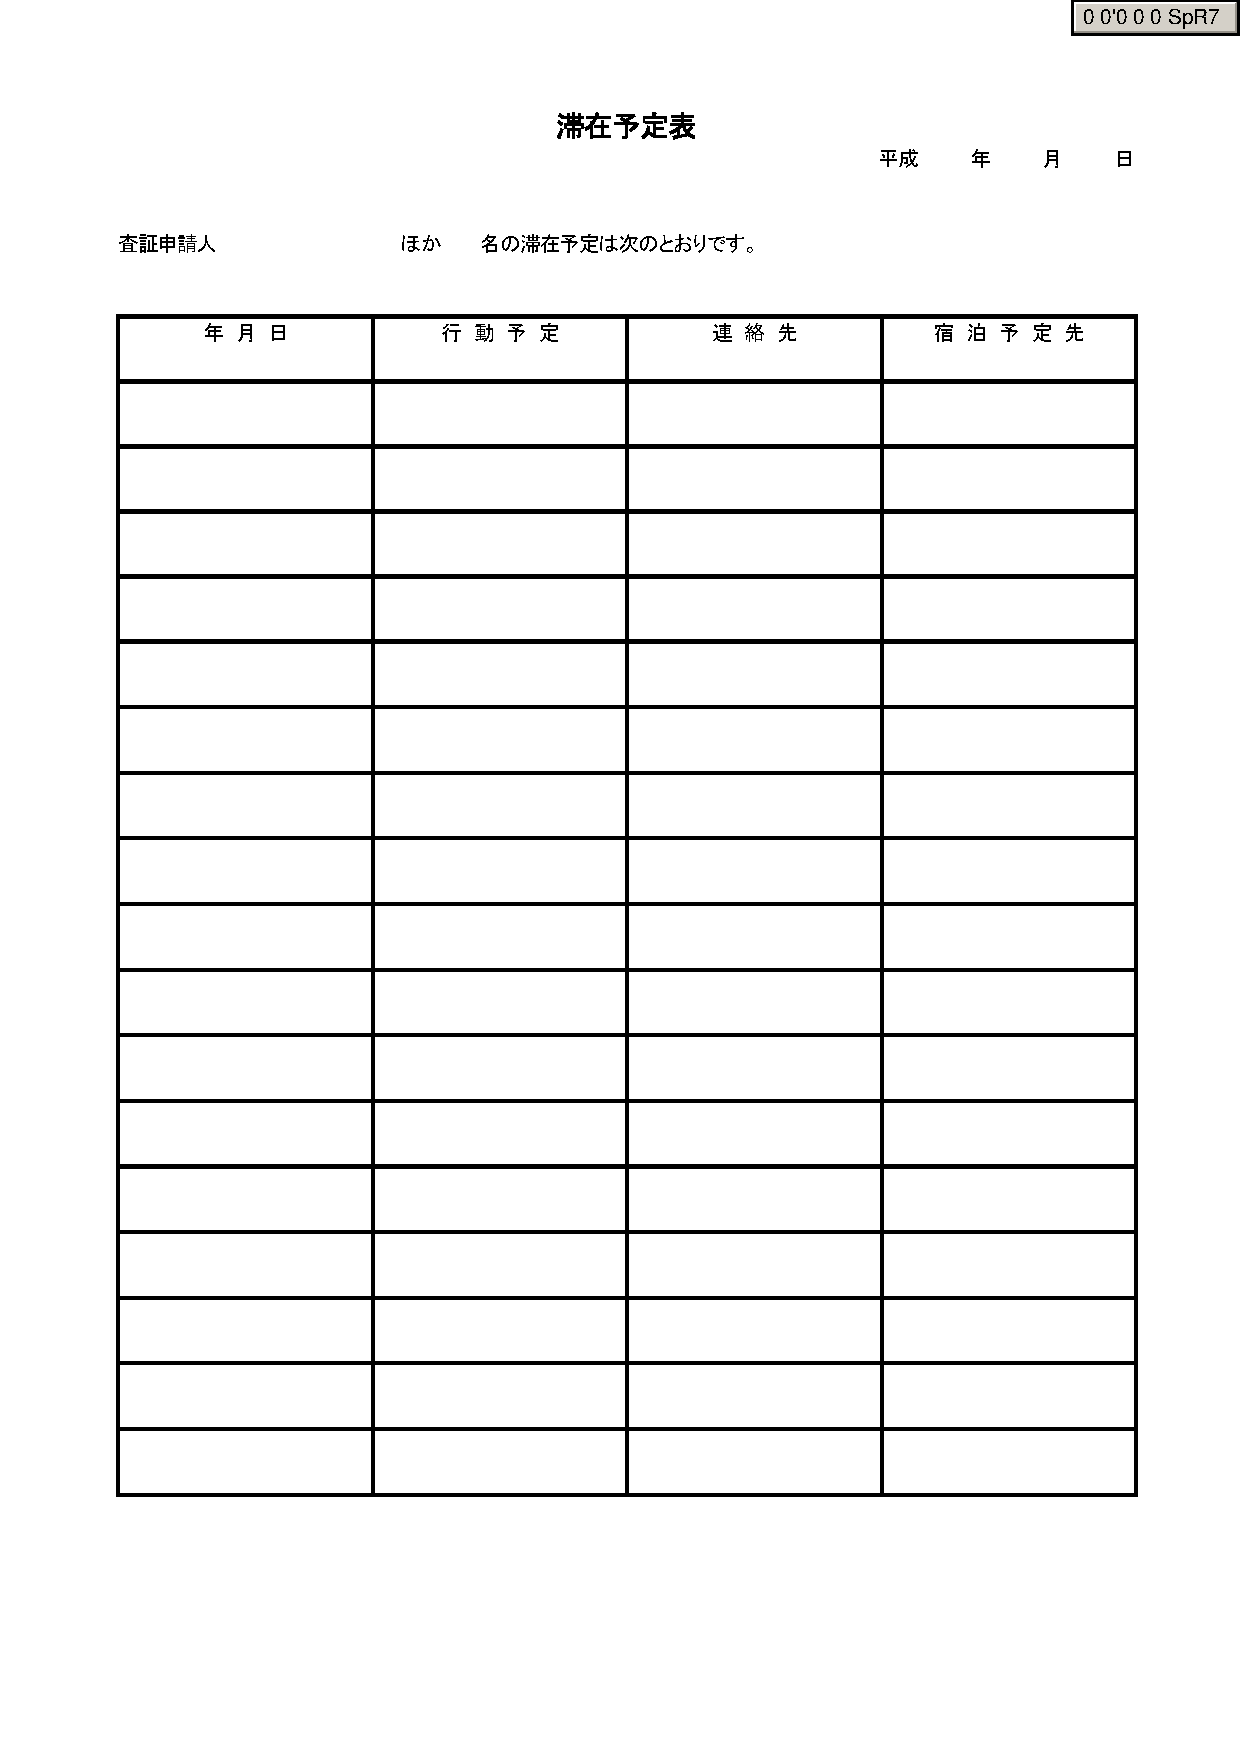
\includegraphics{000262563.pdf}}
\vspace{2.3cm}
\hspace{15.7cm}\平成\hspace{1.2cm}\月\hspace{0.8cm}\日 \hfill \\[0.95cm]
\hspace{4.5cm}{\small \氏名}\\
\ \\[1.7cm]
\hspace{2.75cm}\vbox{\noindent
\スケジュール
}
\clearpage
\vbox to 0in{\includegraphics{\letterheadfile}}
\vspace{\letterheadheight}
\noindent
\hspace{14mm}\fixedbox{16cm}{20cm}{
\begin{flushright}
\日 \月英語, \西暦
\end{flushright}
\begin{flushleft}
Name:  \氏名 \\
Affiliation: \所属 \\
\end{flushleft}

Dear \称号 \氏名,
\bigskip

\招待状
}


\end{document}

